\section{Box dimension in detail}\label{app:dimension}

\subsection{Classes, windows and data}

\paragraph{End box.} The correction of the end box moves $D$ from \DmCrAlpsFromBoxRaw{} to \DmCrAlpsFromBox{} in the Alps on the window from 0.1~km (column \code{D\_box\_raw} of \code{out/dimension/dimension\_windows.csv}).

\paragraph{Pooling.} Curves are pooled in length classes. A class holds the curves of at least $L_{\min}$ and the box sizes $\varepsilon\le L_{\min}/\DmRatio$, so that the same curves are used at every scale of the class.
$N-1$ and $L$ are divided by the length of each curve and averaged with equal weight per curve. The classes are $L_{\min}=2,4,8,16,32,64$~km. Pieces of a route shorter than \DmMinPieceKm~km are not counted.

\paragraph{Windows and $1/H$.} The windows of arc length $s$ are those of Table~\ref{tab:hgeo}. A window $[s_1,s_2)$ becomes the box sizes
$\varepsilon_1=\max(\DmEpsMin~\mathrm m,\sqrt{\mathrm{MSD}(s_1)})$ to $\varepsilon_2=\sqrt{\mathrm{MSD}(s_2)}$, with the MSD of all the paths of the region. We use the smallest class that reaches $\varepsilon_2$ and holds at least
\DmMinGroups{} trees; if none does, the largest such class and the part of the window it reaches. $D$ and $1/H$ are then computed on the same curves and the same range: $H$ is the slope of $\ln\mathrm{MSD}$ against $\ln s$ of the curves of the class
between the $s$ that the chord assigns to the first and the last box size. The routes use the class and the box sizes of the crests of the same massif. The window from 0.1~km uses the class of at least \DmCrAlpsFromClassKm~km.

\paragraph{Data and intervals.} The crests are the \CgAlpsPaths{} and \CgPyrPaths{} paths of $\Hgeo$, in the same order as their TAMSD rows. The routes are those of the paragliding flights of Section~\ref{sec:flights}
(declared distance flights, opening at least \DmOpening): a smoothing spline resampled every \DmStep~m of arc length with the climb phases replaced by their chords, \DmFlightsAlps{} flights in the Alps and \DmFlightsPyr{} in the Pyrenees
with a piece of at least \DmMinPieceKm~km. The intervals are 95\% bootstrap intervals from \DmBoot{} resamples of whole trees for the crests and whole flights for the routes. The difference of two quantities of the same curves uses the same resample;
the difference between crests and routes uses independent resamples.

\subsection{The window from 0.1 to 1~km}

Table~\ref{tab:dimshort} gives the window left out of Table~\ref{tab:dim}, on the boxes that the chord assigns to it. The intervals of $D_{\mathrm{box}}$, $D_{\mathrm{div}}$ and $1/H$ themselves are in
\code{out/dimension/dimension\_windows.csv}.

\begin{table}[H]
\centering
\caption{As Table~\ref{tab:dim} for the window from 0.1 to 1~km. The box sizes translate the window of arc length by the chord.}
\label{tab:dimshort}
\small
\setlength{\tabcolsep}{4pt}
\begin{tabular}{lccccc}
\toprule
window of $s$ & $D_{\mathrm{box}}$ & $D_{\mathrm{div}}$ & $1/H$ & $D_{\mathrm{box}}-1/H$ & $D_{\mathrm{div}}-1/H$ \\
\midrule
\textit{Alps crests} & & & & & \\
0.1--1~km & 1.034 & 1.051 & 1.044 & \ensuremath{-}0.011 (\ensuremath{-}0.012, \ensuremath{-}0.009) & 0.006 (0.005, 0.007) \\
\midrule
\textit{Pyrenees crests} & & & & & \\
0.1--1~km & 1.035 & 1.052 & 1.046 & \ensuremath{-}0.011 (\ensuremath{-}0.013, \ensuremath{-}0.010) & 0.006 (0.005, 0.007) \\
\midrule
\textit{Alps routes} & & & & & \\
0.1--1~km & 1.072 & 1.093 & 1.068 & 0.003 (0.003, 0.004) & 0.024 (0.024, 0.025) \\
\midrule
\textit{Pyrenees routes} & & & & & \\
0.1--1~km & 1.079 & 1.095 & 1.070 & 0.009 (0.007, 0.011) & 0.025 (0.024, 0.027)
\\
\bottomrule
\end{tabular}
\end{table}

\subsection{A fixed population against all the curves}

The windows of $1/H$ of Table~\ref{tab:hgeo}, fitted on all the curves, give another picture for the window from 0.1~km in the Alps: $1/\Hgeo=\DmCrAlpsFromStdInvH$ (\DmCrAlpsFromStdInvHLo, \DmCrAlpsFromStdInvHHi) for the crests and
$1/\Hroute=\DmRtAlpsFromStdInvH$ (\DmRtAlpsFromStdInvHLo, \DmRtAlpsFromStdInvHHi) for the routes, so the routes look smoother than the crests. Each lag of those fits uses the curves long enough for it, so the small lags see mostly short curves
and the large lags long ones, and the two groups do not have the same mix of curves. With the population fixed on the long curves the crests have $1/H=\DmCrAlpsFromInvH$ and the routes $\DmRtAlpsFromInvH$, so the routes are rougher.
The dimension needs a fixed population, so these are the values to compare.

\subsection{Joins and smoothing}

Two steps of the construction could bring $D$ towards 1: the smoothing of the curves with a cut-off of 100~m and the straight joins of up to 1~km. The fits start at \DmEpsMin~m, above the cut-off. For the joins, Table~\ref{tab:dimcurves}
gives $D$ and $1/H$ for the curves alone, before the joins, and for the paths, on the same box sizes and the same minimum length. The curves alone are shorter, so only the lowest boxes are available.

\begin{table}[H]
\centering
\caption{Paths and curves (no joins) of at least 4 and 8~km, on the box sizes up to $L_{\min}/\DmRatio$.}
\label{tab:dimcurves}
\footnotesize
\setlength{\tabcolsep}{3pt}
\begin{tabular}{llcccc}
\toprule
 & $\varepsilon$ (km) & curves & $D_{\mathrm{box}}$ & $D_{\mathrm{div}}$ & $1/H$ \\
\midrule
\textit{Alps} & & & & & \\
paths, $\ge4$~km & 0.20--0.43 & 10\,975 & 1.029 (1.027, 1.031) & 1.046 (1.044, 1.047) & 1.040 (1.039, 1.041) \\
curves, $\ge4$~km & 0.20--0.43 & 1\,795 & 1.029 (1.027, 1.031) & 1.031 (1.030, 1.032) & 1.028 (1.027, 1.029) \\
paths, $\ge8$~km & 0.20--0.93 & 8\,949 & 1.037 (1.035, 1.039) & 1.053 (1.051, 1.055) & 1.047 (1.045, 1.048) \\
curves, $\ge8$~km & 0.20--0.93 & 181 & 1.031 (1.028, 1.034) & 1.032 (1.030, 1.034) & 1.028 (1.027, 1.030) \\
\midrule
\textit{Pyrenees} & & & & & \\
paths, $\ge4$~km & 0.20--0.43 & 5\,409 & 1.027 (1.025, 1.031) & 1.046 (1.044, 1.049) & 1.040 (1.038, 1.042) \\
curves, $\ge4$~km & 0.20--0.43 & 944 & 1.029 (1.027, 1.032) & 1.033 (1.032, 1.035) & 1.030 (1.029, 1.031) \\
paths, $\ge8$~km & 0.20--0.93 & 4\,413 & 1.037 (1.035, 1.040) & 1.055 (1.052, 1.057) & 1.049 (1.047, 1.051) \\
curves, $\ge8$~km & 0.20--0.93 & 73 & 1.035 (1.030, 1.041) & 1.038 (1.034, 1.042) & 1.031 (1.029, 1.034)
\\
\bottomrule
\end{tabular}
\end{table}

The box dimension of the curves alone equals that of the paths (\DmJnAlpsFourCurvesBox{} and \DmJnAlpsFourPathsBox{} in the Alps at 4~km). The divider dimension and $1/H$ of the paths are higher, by \DmJnAlpsFourDivGap{} for the divider at
4~km in the Alps. So the joins do not pull $D$ down. The smoothing cannot be tested with this elevation model. It sets a floor: below its cut-off any curve has $D=1$, and the local dimension of Figure~\ref{fig:dimscales} starts at
\DmLocAlpsCrBoxLo{} at \DmEpsMin~m in the Alps. The values at the lowest boxes can be too low.

\subsection{The literature}

\paragraph{A single line.} Fehr et al.\ measured the main watershed of the Alps, one line between two sinks computed on SRTM at 90~m, with the divider method over 100~m to 200~km: $D=\DmFehrAlps\pm0.01$~\cite{fehr}. This is a single-curve
dimension, as ours. The divider dimension of our \DmNLongest{} longest paths of the Alps (\DmLongAlpsLenMinKm{} to \DmLongAlpsLenMaxKm~km), fitted from \DmEpsMin~m to the length over \DmRatio, has a mean of \DmLongAlpsDivMean{} (from \DmLongAlpsDivMin{}
to \DmLongAlpsDivMax{} over the paths); the ten paths come from \DmLongAlpsTrees{} trees and overlap. The pooled paths of at least 64~km, boxes up to \DmPoolAlpsEpsHiKm~km, give \DmPoolAlpsDiv{} (\DmPoolAlpsDivLo, \DmPoolAlpsDivHi).
Our range of scales ends at \DmLongAlpsEpsHiKm~km, against 200~km, and the two lines are of different kinds (a watershed between two sinks, a divide of a network); the values are close.

\paragraph{A network.} Rak et al.\ extracted the ridge axes of the Alps and the Pyrenees on SRTM (3 arc seconds), joined them in a tree and counted boxes of the whole map~\cite{rak}: $D=\DmRakAlpsSmall$ (Alps) and $\DmRakPyrSmall$ (Pyrenees)
for boxes of 1 to 16 pixels (\DmRakSmallPixLoM~m to \DmRakSmallHiKm~km), and $\DmRakAlpsLarge$ and $\DmRakPyrLarge$ for 32 to 4096 pixels, where the map fills the plane. This is a network dimension, with the branching included, and it is not comparable
with $1/H$ of a single path. The right comparison is with the box counting of the union of all our crest curves of a massif (Figure~\ref{fig:dimnet}, \DmNetAlpsPoints{} points in the Alps), fitted on the same ranges: boxes of \DmEpsMin~m to
\DmRakSmallHiKm~km and of \DmRakLargeLoKm~km to \DmRakLargeHiKm~km.

\begin{figure}
\centering
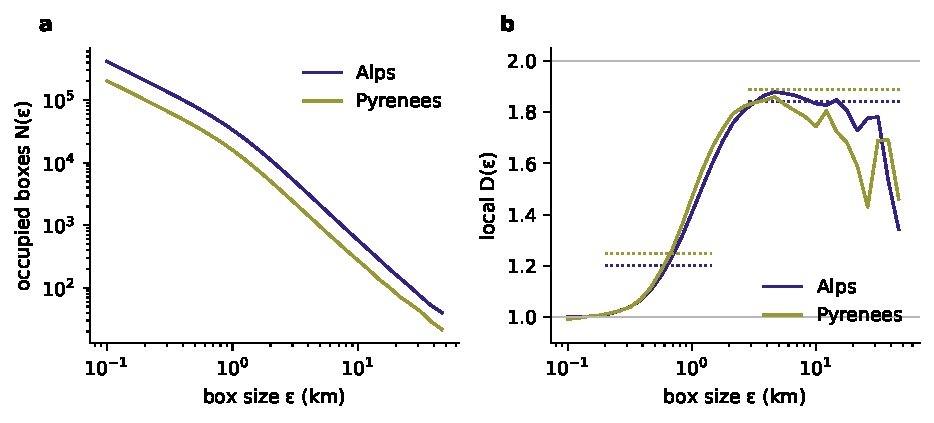
\includegraphics[width=\textwidth]{figures/dimension_network.pdf}
\caption{The network of the crests has the dimension of a network. Box counting of the union of the crest curves of a massif. \textbf{a}~Occupied boxes $N(\varepsilon)$. \textbf{b}~Local dimension; dotted lines: the values of Rak et al.\ on their two ranges.}
\label{fig:dimnet}
\end{figure}

On the small boxes we find \DmNetAlpsSmall{} in the Alps and \DmNetPyrSmall{} in the Pyrenees, against \DmRakAlpsSmall{} and \DmRakPyrSmall. On the large boxes we find \DmNetAlpsLarge{} and \DmNetPyrLarge, against \DmRakAlpsLarge{} and
\DmRakPyrLarge. A single line and a network differ because a network has many strands. At the smallest boxes a box holds one strand and the local dimension is that of the strand, \DmNetAlpsLocLo{} at \DmEpsMin~m in the Alps. Once a box is larger
than the distance between two crests it holds several strands and the dimension goes to 2. The value on the small boxes is an average over the climb between the two and depends on the range chosen. Our local dimension crosses 1.5 at a box of
\DmNetAlpsCross~km in the Alps and \DmNetPyrCross~km in the Pyrenees and reaches \DmNetAlpsMax{} and \DmNetPyrMax. It then falls above 10~km, where the boxes reach the size of the massif and its edge. Our small-box value is lower than that of
Rak et al.: our fit starts at \DmEpsMin~m instead of \DmRakSmallPixLoM~m, our curves are smoothed at 100~m, are at least 1~km long and are divides only, while their axes come from a 90~m grid and contain small branches. On the large boxes the
Alps are close to their value and the Pyrenees are lower than theirs.
